\chapter{Sprint 4 : détection intelligente d'anomalies, conception, intégration et évaluation}
\label{ch:sprint4}
\startcontents[chapters]
\chapterplan

\section{Introduction}

Les contrôles métier et la validation XSD détectent les erreurs que l'on sait formuler. Ils ne signalent pas un montant plausible mais anormal pour un salarié donné, ni une fiche dont aucune règle simple ne trahit le défaut. Le quatrième sprint ajoute cette couche d'analyse : un module d'intelligence artificielle, indépendant du backend, qui attribue à chaque paiement un score d'atypie, explique ses signalements et propose une action. Planifié sur quatre semaines (tableau~\ref{tab:sprints}), il couvre les récits US17 à US20 (tableau~\ref{tab:backlog}).

Ce chapitre est le plus important du rapport sur le plan scientifique, car il ne se contente pas de décrire une fonction : il mesure ce qu'elle apporte. Il présente la conception et l'intégration du module, puis son évaluation sur un jeu de données réaliste et reproductible, afin de répondre à trois questions : quelle est la qualité de détection du modèle en service, quelles améliorations sont possibles, et quelle valeur l'IA ajoute-t-elle aux règles métier ?

\section{Conception du module d'IA}

\subsection{Cas d'utilisation}

La figure~\ref{fig:uc-s4} présente les cas d'utilisation du sprint. L'Expert RH déclenche l'analyse lorsqu'il lance un contrôle, puis consulte les fiches suspectes ; le Manager retrouve les mêmes informations au moment de décider. Les deux profils métier traitent les anomalies et suivent les indicateurs d'apport de l'IA. L'administrateur supervise le module et peut le réentraîner, sans accéder aux données individuelles de paie.

\begin{figure}[H]
\centering
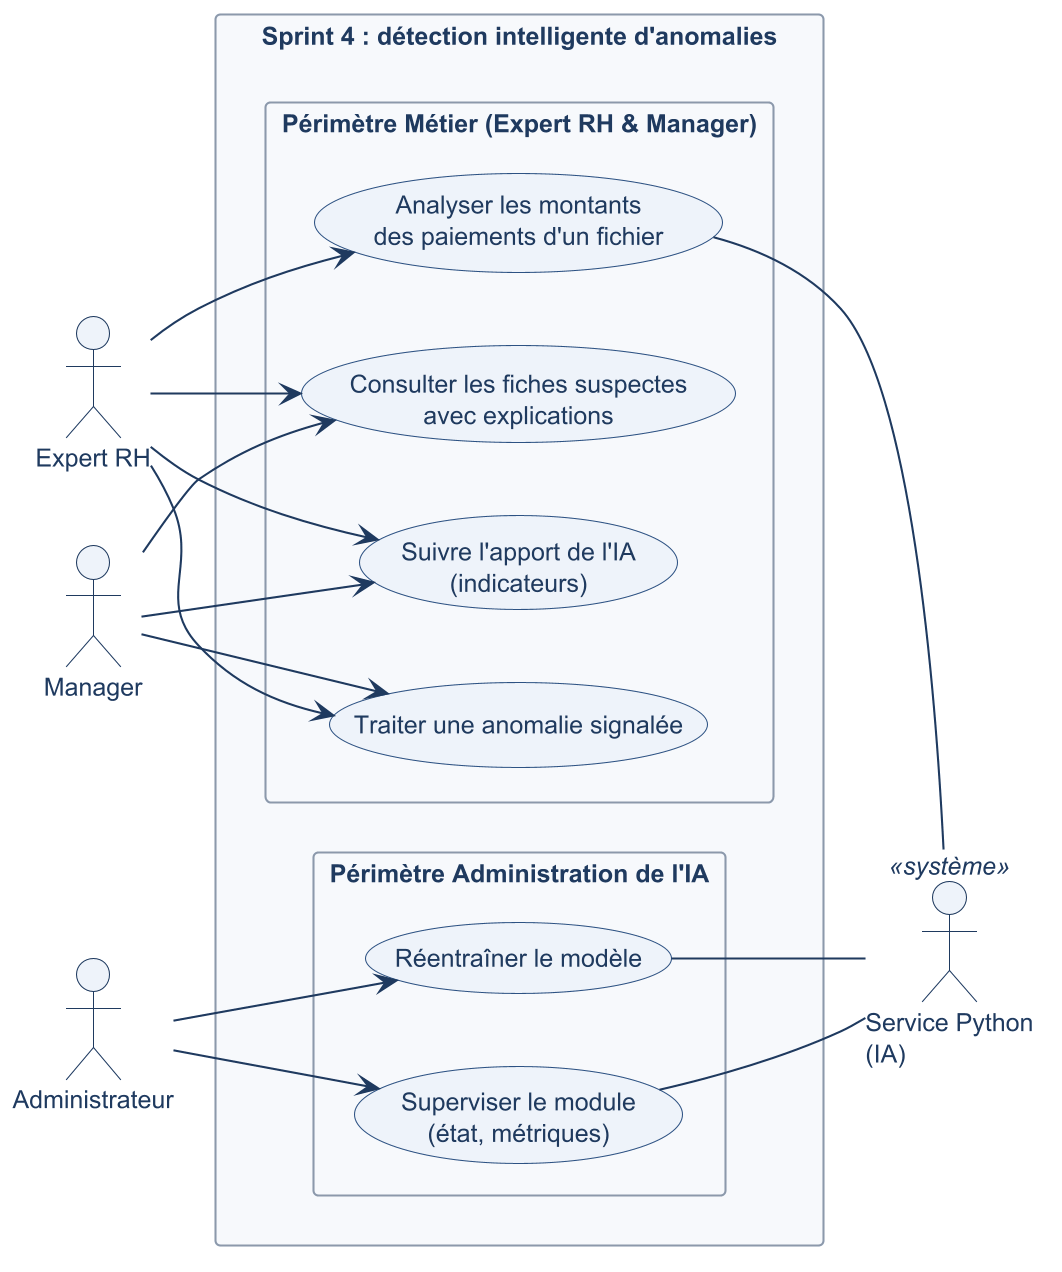
\includegraphics[height=0.33\textheight,width=\textwidth,keepaspectratio]{fig7_1_cas_utilisation_sprint4}
\caption{Cas d'utilisation du sprint 4}
\label{fig:uc-s4}
\end{figure}

\subsection{Principe : une aide à la décision, non un juge}

Quatre principes guident la conception. Le module est \textbf{indépendant} : il s'exécute dans un service Python distinct, ce qui permet d'utiliser l'écosystème d'apprentissage automatique sans alourdir le backend (chapitre~\ref{ch:architecture}). Il est \textbf{non bloquant} : son absence ne doit jamais empêcher un contrôle d'aboutir. Il est \textbf{explicable} : chaque signalement est accompagné de raisons lisibles. Enfin, il reste une \textbf{aide à la décision} : il signale, l'utilisateur tranche. Un signalement ne rejette jamais un paiement ; il produit un avertissement, comme le prévoit le chapitre~\ref{ch:sprint3}.

\subsection{Échange entre le backend et le service Python}

Le service Python n'accède pas à la base de données. Le backend lui transmet, pour chaque paiement à analyser, l'identifiant de la fiche, le montant, l'IBAN, l'historique des montants du salarié sur les six derniers mois, du plus ancien au plus récent, et un indicateur précisant si l'IBAN diffère de celui du paiement précédent. La figure~\ref{fig:seq-ia} illustre cet échange.

\begin{figure}[H]
\centering
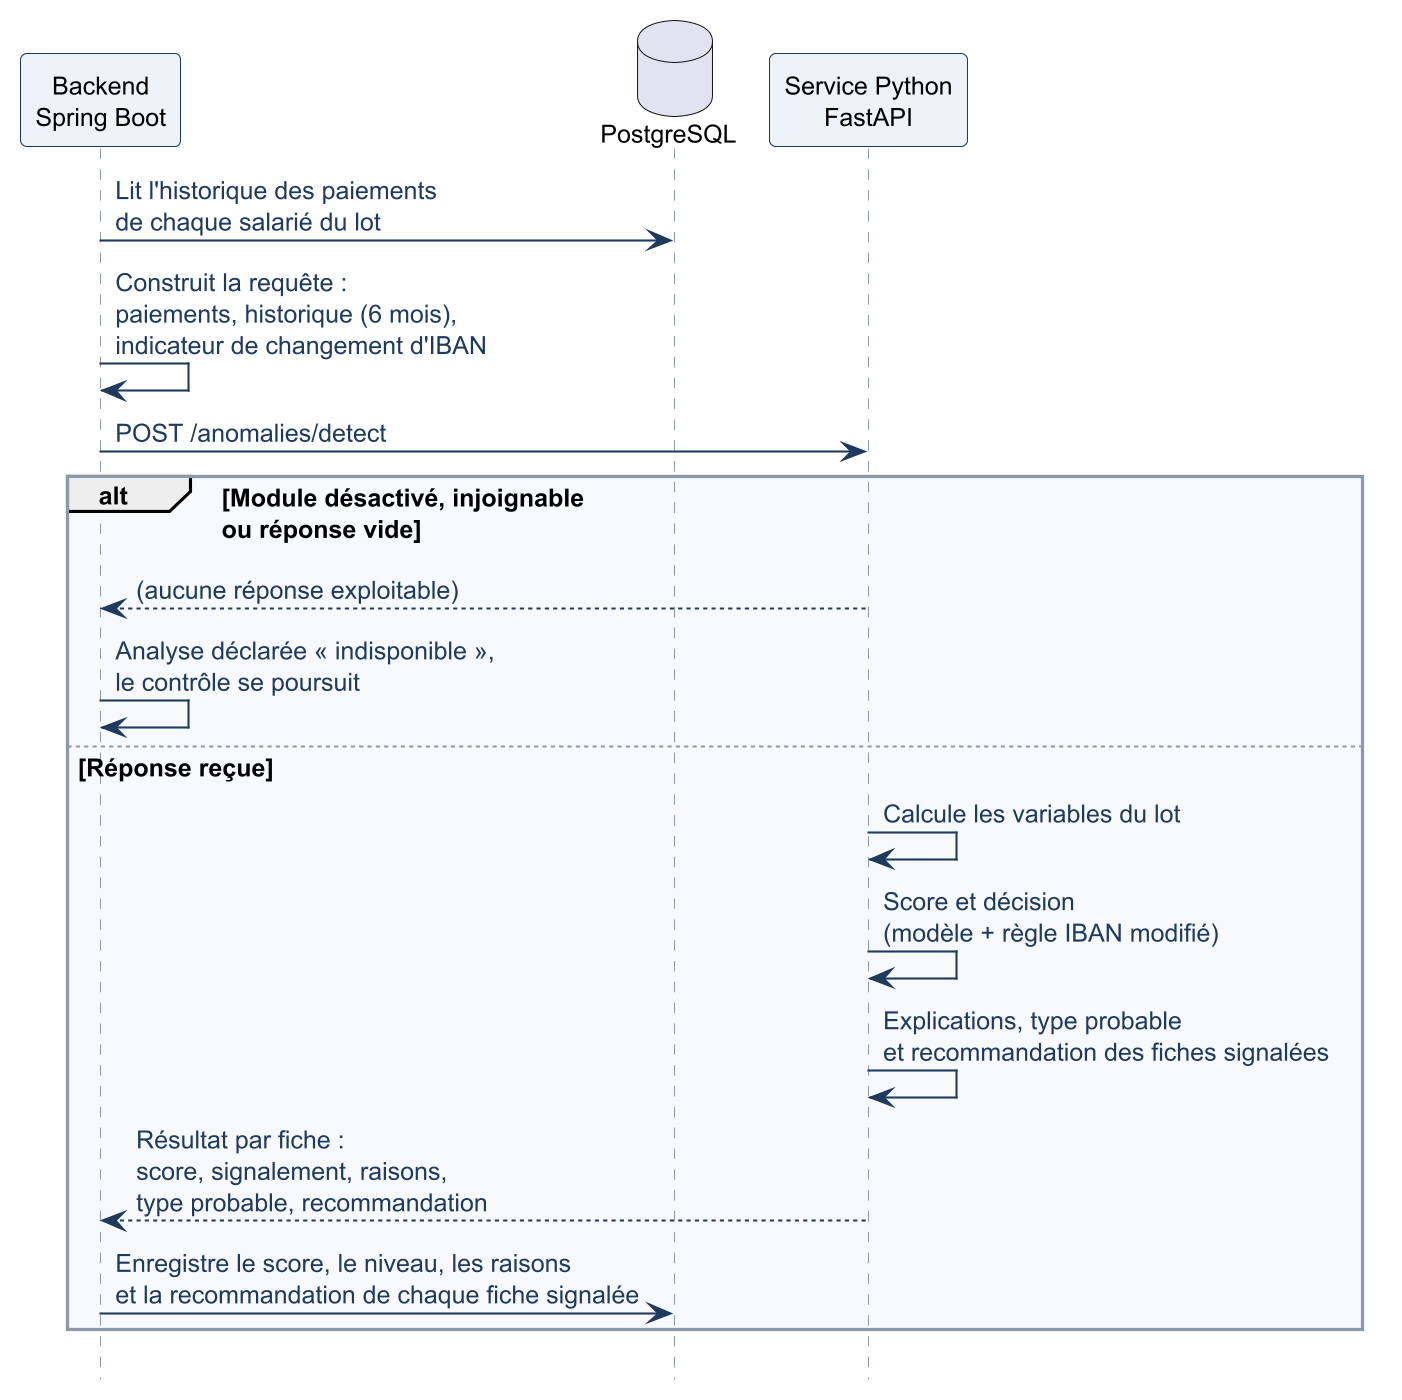
\includegraphics[height=0.5\textheight,width=\textwidth,keepaspectratio]{fig7_2_sequence_analyse}
\caption{Séquence d'analyse d'un lot de paiements}
\label{fig:seq-ia}
\end{figure}

Le client HTTP du backend est configuré avec un délai court de cinq secondes. Toute erreur (module désactivé, injoignable, trop lent, réponse vide) est capturée, consignée dans les journaux techniques et traduite en un résultat \og analyse indisponible\fg{}. Aucune exception ne remonte au traitement appelant. Le résultat d'un contrôle indique alors explicitement que l'IA n'a pas été exécutée, afin qu'une absence d'analyse ne soit jamais confondue avec une absence de risque.

\subsection{Variables comportementales}

Le modèle ne reçoit pas les données brutes d'identité. Il apprend à partir de six variables calculées pour chaque paiement, résumées dans le tableau~\ref{tab:variables-ia}. Elles comparent le paiement à l'historique du salarié et aux autres paiements du lot analysé, car un même montant peut être normal pour un dirigeant et suspect pour un employé.

\begin{table}[H]
\centering
\small
\renewcommand{\arraystretch}{1.2}
\tablestyle
\begin{tabularx}{\textwidth}{|>{\raggedright\arraybackslash}p{4.4cm}|Y|}
\hline
\rowcolor{appMarine}\entete{Variable} & \entete{Description} \\
\hline
Montant & Montant du paiement \\
\hline
Écart à la moyenne du salarié & Rapport entre le montant et la moyenne de ses six derniers paiements (neutre en l'absence d'historique) \\
\hline
Écart dans le lot (\textit{z-score}) & Position du montant par rapport aux autres paiements du lot, en nombre d'écarts-types \\
\hline
Variation sur le mois précédent & Variation relative par rapport au paiement précédent \\
\hline
IBAN modifié & Vaut un si l'IBAN diffère de celui du paiement précédent \\
\hline
Paiements sur le même IBAN & Nombre de paiements du lot versés sur le même IBAN \\
\hline
\end{tabularx}
\caption{Variables du modèle de détection}
\label{tab:variables-ia}
\end{table}

Trois autres calculs servent uniquement à \textbf{expliquer} un signalement et n'alimentent pas le modèle : le nombre de fiches strictement identiques (même salarié, même IBAN, même montant), le nombre de salariés distincts partageant un IBAN, et l'absence d'historique.

\subsection{Isolation Forest, score et niveaux de risque}

Le modèle est un \textbf{Isolation Forest} (200 arbres, proportion d'anomalies attendue de 1~\%) appliqué après une mise à l'échelle des variables. Son principe a été présenté au chapitre~\ref{ch:architecture} : les observations atypiques sont isolées plus vite par des partitions aléatoires. Le score brut est transformé en une valeur comprise entre 0 et 1, d'autant plus élevée que le paiement est atypique.

La décision de signalement combine trois conditions : la prédiction native du modèle, un score au moins égal au seuil configuré, ou un changement d'IBAN. Cette dernière règle est volontairement explicite : l'évaluation a montré que le modèle seul ne repère pas un changement d'IBAN lorsque le montant reste normal, alors que ce cas mérite toujours une vérification auprès du salarié. Le score est ensuite converti en un niveau de risque : \textbf{faible} sous 0,35, \textbf{moyen} de 0,35 à 0,6 et \textbf{élevé} au-delà ; le niveau \og critique\fg{} de la fiche de paie (à partir de 0,85) est fondu dans \og élevé\fg{} dans l'affichage du contrôle.

La figure~\ref{fig:pipeline} résume la chaîne de traitement.

\begin{figure}[H]
\centering
\begin{tikzpicture}[
  etape/.style={draw=appMarine, fill=appClair, rounded corners=3pt, align=center, text width=2.9cm, minimum height=1.5cm, font=\small, execute at begin node={\hyphenpenalty=10000\relax}},
  fleche/.style={-{Stealth[length=2.4mm]}, appMarine, thick}]
\node[etape] (a) {Paiements du lot\\et historique};
\node[etape, right=0.55cm of a] (b) {Calcul des\\six variables};
\node[etape, right=0.55cm of b] (c) {Isolation Forest\\et score de 0 à 1};
\node[etape, below=0.8cm of a] (d) {Décision :\\modèle, seuil,\\IBAN modifié};
\node[etape, right=0.55cm of d] (e) {Niveau de risque,\\raisons et type\\probable};
\node[etape, right=0.55cm of e] (f) {Recommandation\\et résultat\\renvoyé};
\draw[fleche] (a) -- (b);
\draw[fleche] (b) -- (c);
\draw[fleche] (c.south) -- ++(0,-0.4) -| (d.north);
\draw[fleche] (d) -- (e);
\draw[fleche] (e) -- (f);
\end{tikzpicture}
\caption{Chaîne de traitement du module d'IA}
\label{fig:pipeline}
\end{figure}

\subsection{Entraînement et réentraînement}

Au premier démarrage, faute de données de production, le service entraîne le modèle sur un jeu de paiements synthétiques. Le modèle et ses métadonnées sont enregistrés sur un volume persistant : ils survivent à la recréation des conteneurs. Chaque modèle porte une version horodatée, visible dans les résultats.

L'administrateur peut ensuite réentraîner le modèle, soit sur des données synthétiques, soit sur les paiements réellement enregistrés. Dans le second cas, les fiches dont une anomalie d'origine IA a été confirmée par un utilisateur sont exclues, afin que le modèle apprenne ce qui est normal à partir de données vérifiées ; l'opération est refusée si moins de cent paiements sont exploitables. Après chaque entraînement, le service évalue le nouveau modèle en tâche de fond sur un jeu synthétique interne, sans retarder la réponse. Ces opérations sont exposées par des points d'accès d'administration ; elles ne disposent pas d'écran dédié dans l'interface actuelle.

Les retours des utilisateurs alimentent également un indicateur de \textbf{précision observée} : le nombre d'anomalies d'IA confirmées rapporté à celui des anomalies confirmées ou ignorées. Les clôtures automatiques, lorsqu'une anomalie n'est plus détectée, ne comptent pas comme des confirmations.

\subsection{Explications, types probables et recommandations}

Pour chaque paiement signalé, le service produit des raisons en langage clair, un type probable et une recommandation. Ces éléments ne proviennent pas d'un modèle de langage : ils sont déduits de seuils explicites appliqués aux variables du paiement, ce qui les rend prévisibles et vérifiables. Par exemple, une raison peut être \og Montant 3,1$\times$ la moyenne des 6 derniers mois\fg{} ou \og IBAN modifié ce mois-ci\fg{}.

Le type probable est le premier critère satisfait dans un ordre fixe, du plus certain au plus général : montant nul ou négatif, doublon, IBAN partagé, IBAN modifié avec montant élevé, IBAN modifié, salarié sans historique, erreur de virgule, montant très supérieur à l'habituel, hausse ou baisse inhabituelle, puis un type générique lorsque le modèle signale une fiche sans qu'aucun critère particulier ne soit satisfait. Chaque type est associé à une recommandation adaptée, par exemple demander un RIB signé pour un changement d'IBAN ou contrôler la saisie en cas de décalage de virgule probable. Les critères et les recommandations sont détaillés en annexe~\ref{ann:recommandations}.

\section{Intégration dans l'application}

\subsection{Contrôle IA d'un fichier}

L'analyse est exécutée lors du contrôle d'un fichier, après les contrôles métier et avant la génération du XML, sur les paiements sélectionnés (chapitre~\ref{ch:sprint3}). Son résultat est conservé avec le fichier : l'Expert RH et le Manager consultent donc exactement les mêmes constats. La synthèse du résultat comporte une carte \og Contrôle IA\fg{} indiquant le nombre de fiches suspectes sur le nombre de fiches analysées, leur proportion, la version du modèle et la répartition par type probable (figure~\ref{fig:synthese-ia}).

\begin{figure}[H]
\centering
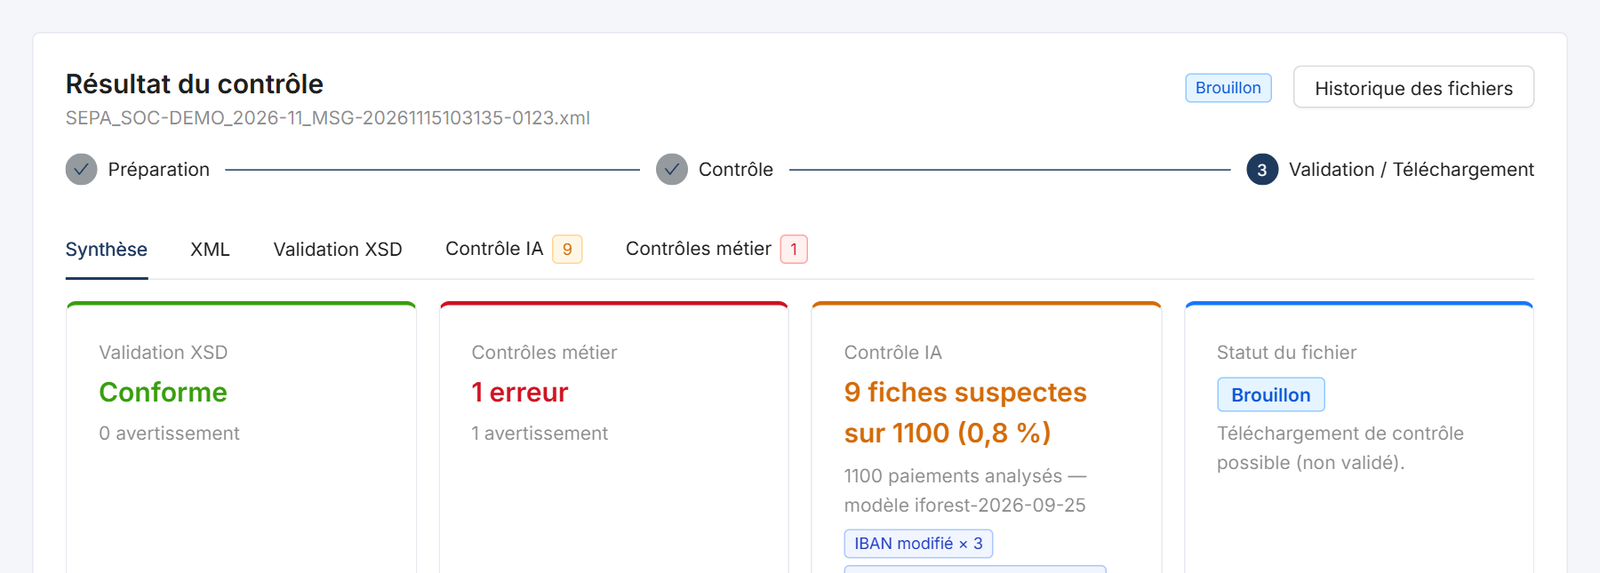
\includegraphics[width=0.95\textwidth]{fig7_synthese_ia}
\caption{Carte \og Contrôle IA\fg{} de la synthèse d'un fichier (scénario de démonstration)}
\label{fig:synthese-ia}
\end{figure}

L'onglet \og Contrôle IA\fg{} détaille chaque fiche suspecte : score et niveau, type probable, explication et recommandation (figure~\ref{fig:controle-ia}). Le tableau est trié par score décroissant et peut être filtré par niveau. L'utilisateur sait ainsi quoi vérifier et pourquoi, ce qui accélère la décision et la rend traçable.

\begin{figure}[H]
\centering
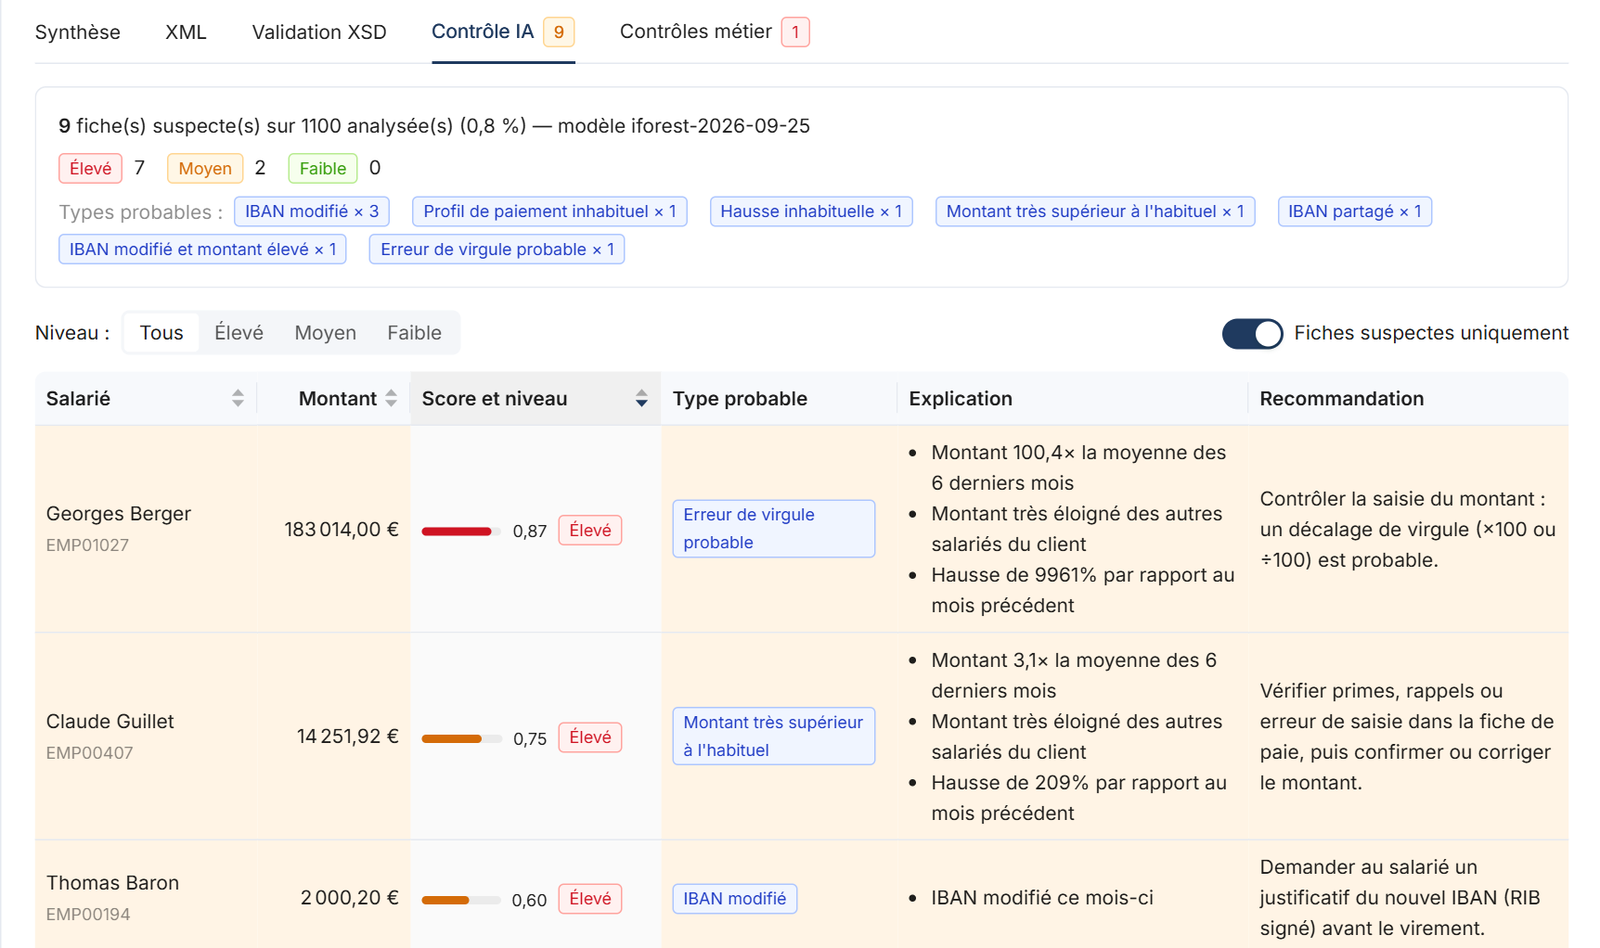
\includegraphics[width=0.95\textwidth]{fig7_controle_ia}
\caption{Onglet \og Contrôle IA\fg{} : fiches suspectes triées par score (scénario de démonstration)}
\label{fig:controle-ia}
\end{figure}

La page des transactions propose aussi une analyse à la demande sur l'ensemble des fiches visibles de l'utilisateur, et le registre des anomalies (chapitre~\ref{ch:sprint3}) intègre les signalements d'origine IA sous le type \texttt{MONTANT\_SUSPECT}.

\subsection{Indicateurs de l'apport de l'IA}

Le tableau de bord des indicateurs affiche deux mesures de l'apport de l'IA sur la période choisie : le nombre de fiches signalées par l'IA, et la \textbf{part détectée par l'IA seule}, c'est-à-dire la proportion de ces fiches que les contrôles métier ne signalent pas (IBAN ou BIC invalide, montant nul ou négatif, doublon). Les chiffres reposent sur la dernière analyse de chaque fiche. En l'absence de fiche signalée, la part n'est pas calculable et s'affiche comme indisponible, et non comme nulle. Pour l'Expert RH, ces indicateurs se limitent à ses sociétés affectées.

\section{Évaluation du modèle}

\subsection{Problématique d'évaluation}

Évaluer un détecteur d'anomalies de paie pose deux difficultés, classiques dans ce domaine~\cite{chandola2009survey}. D'abord, les anomalies sont rares : de l'ordre de 2~\% des fiches. Un modèle qui ne signalerait rien aurait donc une exactitude de 98~\%, sans aucune utilité. Il faut des mesures adaptées au déséquilibre : précision, rappel, F1 et surtout l'aire sous la courbe précision--rappel (PR-AUC), dont la valeur de référence est le taux d'anomalies. La littérature recommande cette courbe plutôt que la courbe ROC lorsque les classes sont très déséquilibrées~\cite{saito2015pr}. Ensuite, nous ne disposons pas de données de paie réelles étiquetées : la paie est confidentielle et les erreurs passées ne sont pas répertoriées. L'évaluation repose donc sur des données \textbf{synthétiques}, dont il faut expliciter les limites.

\subsection{Jeu de données de référence}

Le générateur simule la paie mois par mois. Chaque salarié possède un salaire de base lié à son profil (employé, cadre, dirigeant) et à sa société, un bruit mensuel d'environ 1~\%, une augmentation annuelle en janvier, des promotions occasionnelles, des primes ponctuelles, un 13\textsuperscript{e} mois en décembre pour trois sociétés, des changements d'IBAN légitimes, des entrées et des sorties de personnel. Ces situations normales mais atypiques constituent des \og cas difficiles\fg{} qu'un bon modèle doit laisser passer. Des anomalies de neuf types sont ensuite injectées et étiquetées. Les IBAN générés sont valides et les noms sont fictifs. Une graine fixée rend le jeu reproductible. Le tableau~\ref{tab:jeu-donnees} le décrit.

\begin{table}[H]
\centering
\small
\renewcommand{\arraystretch}{1.15}
\tablestyle
\begin{tabularx}{\textwidth}{|>{\raggedright\arraybackslash}p{7.5cm}|Y|}
\hline
\rowcolor{appMarine}\entete{Caractéristique} & \entete{Valeur} \\
\hline
Sociétés simulées & 9 (de 94 à 1\,159 salariés) \\
\hline
Salariés distincts & 4\,621 \\
\hline
Mois de paie & 18 (juillet 2024 à décembre 2025) \\
\hline
Fiches de paie & 73\,568 \\
\hline
Fiches anormales étiquetées & 1\,517 (2,06~\%), de neuf types \\
\hline
Cas normaux atypiques & 749 primes, 1\,986 versements de 13\textsuperscript{e} mois, 152 changements d'IBAN légitimes \\
\hline
Entraînement (mois 1 à 12) & 48\,791 fiches, 1\,026 anomalies \\
\hline
Validation (mois 13 à 15) & 12\,354 fiches, 242 anomalies \\
\hline
Test (mois 16 à 18) & 12\,423 fiches, 249 anomalies \\
\hline
\end{tabularx}
\caption{Jeu de données synthétique de référence}
\label{tab:jeu-donnees}
\end{table}

Le découpage suit l'ordre du temps : le modèle est entraîné sur les mois 1 à 12, le seuil de décision est choisi sur les mois 13 à 15, et les performances finales sont mesurées sur les mois 16 à 18, jamais utilisés auparavant. Ce protocole reproduit l'usage réel, où l'on contrôle la paie d'un mois à venir avec un modèle appris sur le passé, et évite toute fuite d'information.

La figure~\ref{fig:salaires} justifie le choix de variables relatives : les trois profils occupent des plages de salaire très différentes (médianes d'environ 2\,200~\texteuro{} pour les employés, 4\,200~\texteuro{} pour les cadres et 9\,700~\texteuro{} pour les dirigeants), si bien qu'un seuil global sur le montant serait inopérant.

\begin{figure}[H]
\centering
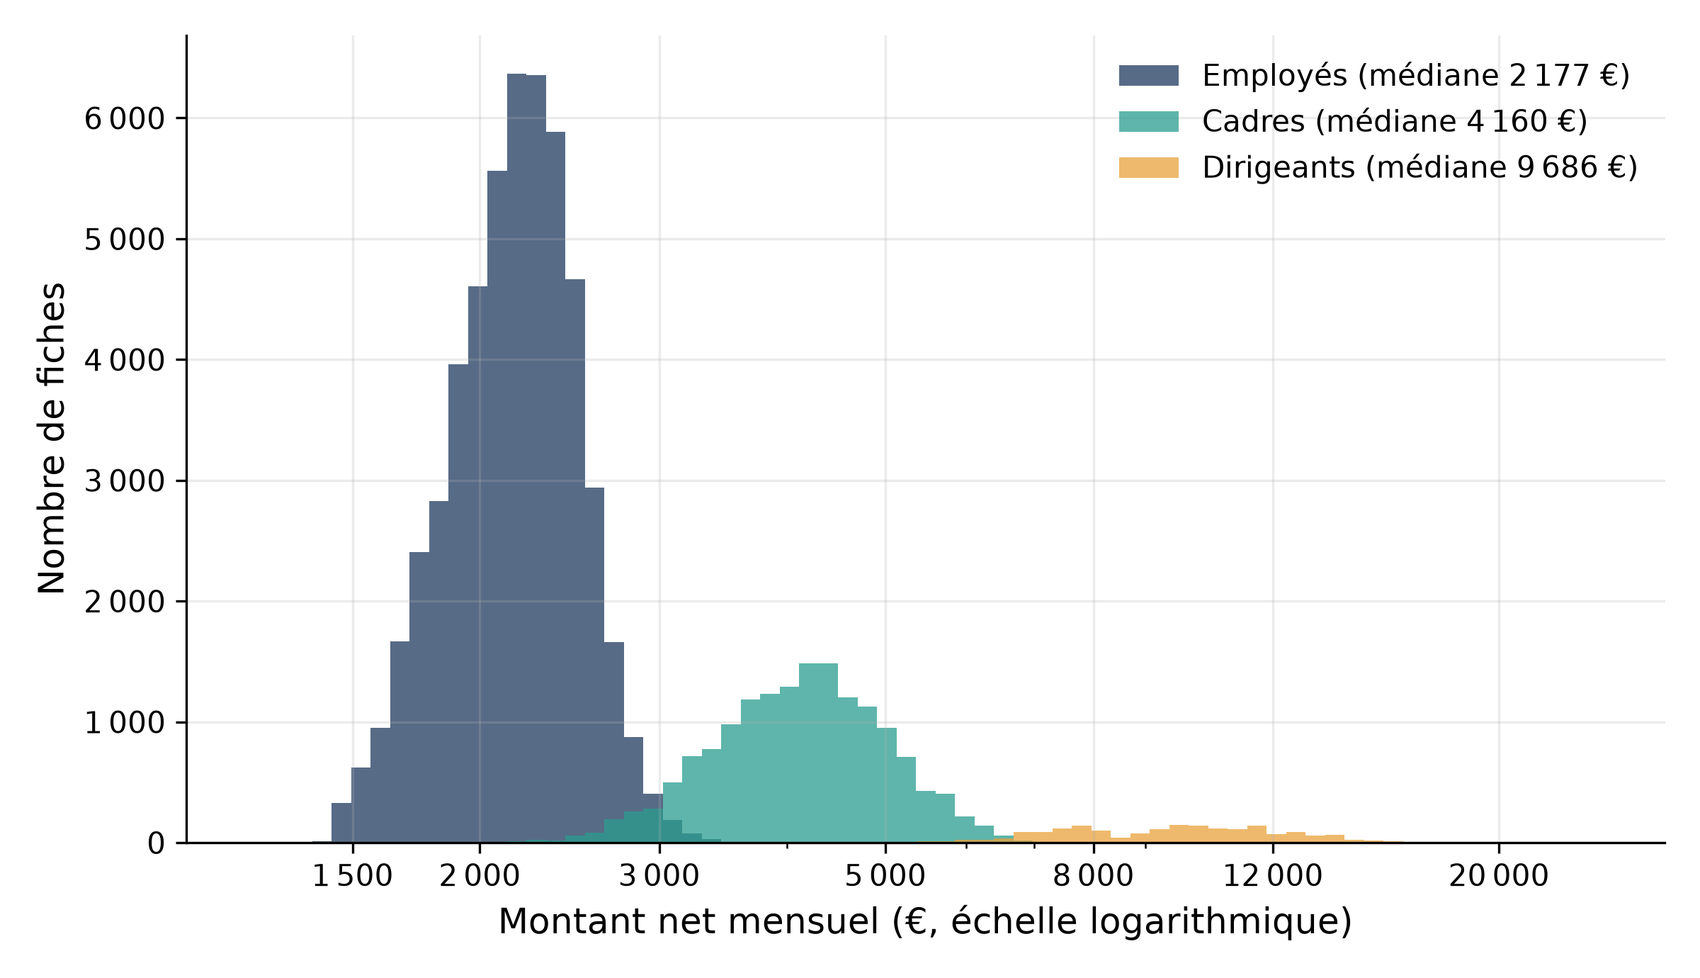
\includegraphics[width=0.85\textwidth]{fig7_salaires}
\caption{Distribution du montant net mensuel selon le profil (fiches normales, hors 13\textsuperscript{e} mois)}
\label{fig:salaires}
\end{figure}

Le tableau~\ref{tab:types-injectes} présente les neuf types d'anomalies injectés, des plus évidents aux plus difficiles. Les doublons et les IBAN partagés étiquettent les deux fiches concernées, car l'Expert RH doit examiner la paire.

\begin{table}[H]
\centering
\small
\renewcommand{\arraystretch}{1.15}
\tablestyle
\begin{tabularx}{\textwidth}{|>{\raggedright\arraybackslash}p{4.9cm}|>{\centering\arraybackslash}p{1.5cm}|Y|}
\hline
\rowcolor{appMarine}\entete{Type d'anomalie} & \entete{Fiches (test)} & \entete{Principe d'injection} \\
\hline
Montant multiplié par 3 à 10 & 24 & Montant légitime multiplié par un facteur tiré entre 3 et 10 \\
\hline
Erreur de virgule & 24 & Montant multiplié ou divisé par 100 \\
\hline
Hausse subtile & 27 & Montant majoré de 25 à 60~\% \\
\hline
Montant nul ou négatif & 35 & Montant égal à zéro ou à l'opposé du montant légitime \\
\hline
Doublon & 26 & Fiche recopiée à l'identique \\
\hline
IBAN modifié et montant élevé & 31 & Nouvel IBAN valide et montant multiplié par 1,5 à 3 \\
\hline
IBAN partagé & 22 & Un salarié reprend l'IBAN d'un collègue \\
\hline
Salarié fantôme & 27 & Salarié sans historique, salaire plausible \\
\hline
Salarié sorti encore payé & 33 & Salarié parti depuis deux à quatre mois, payé à nouveau \\
\hline
\end{tabularx}
\caption{Types d'anomalies injectés}
\label{tab:types-injectes}
\end{table}

\subsection{Protocole et métriques}

Le modèle évalué est celui de l'application, reconstruit avec ses hyperparamètres. Sa décision actuelle est mesurée telle quelle, puis comparée à des variantes dont le seuil est choisi sur la validation en maximisant le F1. Aucun paramètre n'est ajusté en observant le test. Chaque expérience est répétée sur \textbf{cinq graines} (jeu de données et modèle) et rapportée en moyenne $\pm$ écart-type, afin de ne pas conclure sur un tirage favorable. Les mesures retenues sont :
\begin{itemize}
    \item la \textbf{précision} (part des signalements justifiés) et le \textbf{rappel} (part des anomalies retrouvées), résumés par le \textbf{F1} ;
    \item la \textbf{PR-AUC}, mesure principale, comparée au niveau du hasard (2,0~\%) ;
    \item la \textbf{ROC-AUC}, à lire avec prudence car le grand nombre de fiches normales la rend flatteuse~\cite{saito2015pr} ;
    \item le nombre de \textbf{faux positifs pour 1\,000 fiches}, qui traduit la charge de vérification de l'Expert RH.
\end{itemize}

\subsection{Résultats du modèle en service}

Le tableau~\ref{tab:perf-service} présente les performances sur le jeu de test. Avec sa décision actuelle, le modèle atteint une précision de 0,47, un rappel de 0,38 et un F1 de 0,42, pour environ neuf faux positifs sur 1\,000 fiches. Sa PR-AUC de 0,41 est environ 20 fois supérieure à celle d'un classement au hasard : le score contient une réelle information. Elle reste toutefois loin de 1, ce qui signifie que le modèle retrouve environ 38~\% des anomalies et non leur totalité.

\begin{table}[H]
\centering
\footnotesize
\renewcommand{\arraystretch}{1.15}
\tablestyle
\begin{tabularx}{\textwidth}{|>{\raggedright\arraybackslash}p{4.6cm}|Y|Y|Y|Y|Y|}
\hline
\rowcolor{appMarine}\entete{Configuration} & \entete{Précision} & \entete{Rappel} & \entete{F1} & \entete{PR-AUC} & \entete{Faux positifs / 1\,000} \\
\hline
Décision en service (score $\geq$ 0,5 ou IBAN modifié) & 0,47 $\pm$ 0,09 & 0,38 $\pm$ 0,03 & 0,42 $\pm$ 0,05 & 0,41 $\pm$ 0,04 & 8,9 $\pm$ 3,1 \\
\hline
Isolation Forest seul, seuil validé & 0,15 $\pm$ 0,05 & 0,57 $\pm$ 0,09 & 0,23 $\pm$ 0,06 & 0,41 $\pm$ 0,05 & 70,8 $\pm$ 21,2 \\
\hline
Isolation Forest et règle IBAN, seuil validé & 0,16 $\pm$ 0,06 & 0,57 $\pm$ 0,09 & 0,24 $\pm$ 0,07 & 0,33 $\pm$ 0,04 & 68,1 $\pm$ 22,4 \\
\hline
\end{tabularx}
\caption{Performances sur le jeu de test (moyenne $\pm$ écart-type sur cinq graines)}
\label{tab:perf-service}
\end{table}

La figure~\ref{fig:pr-courbe} montre le compromis offert par le score. Les anomalies les mieux classées, jusqu'à un rappel d'environ 0,14, sont retrouvées avec une précision supérieure à 0,95. La précision décroît ensuite à mesure que l'on accepte de signaler davantage de fiches, jusqu'à un palier d'environ 0,12 dû au bloc des 13\textsuperscript{e} mois.

\begin{figure}[H]
\centering
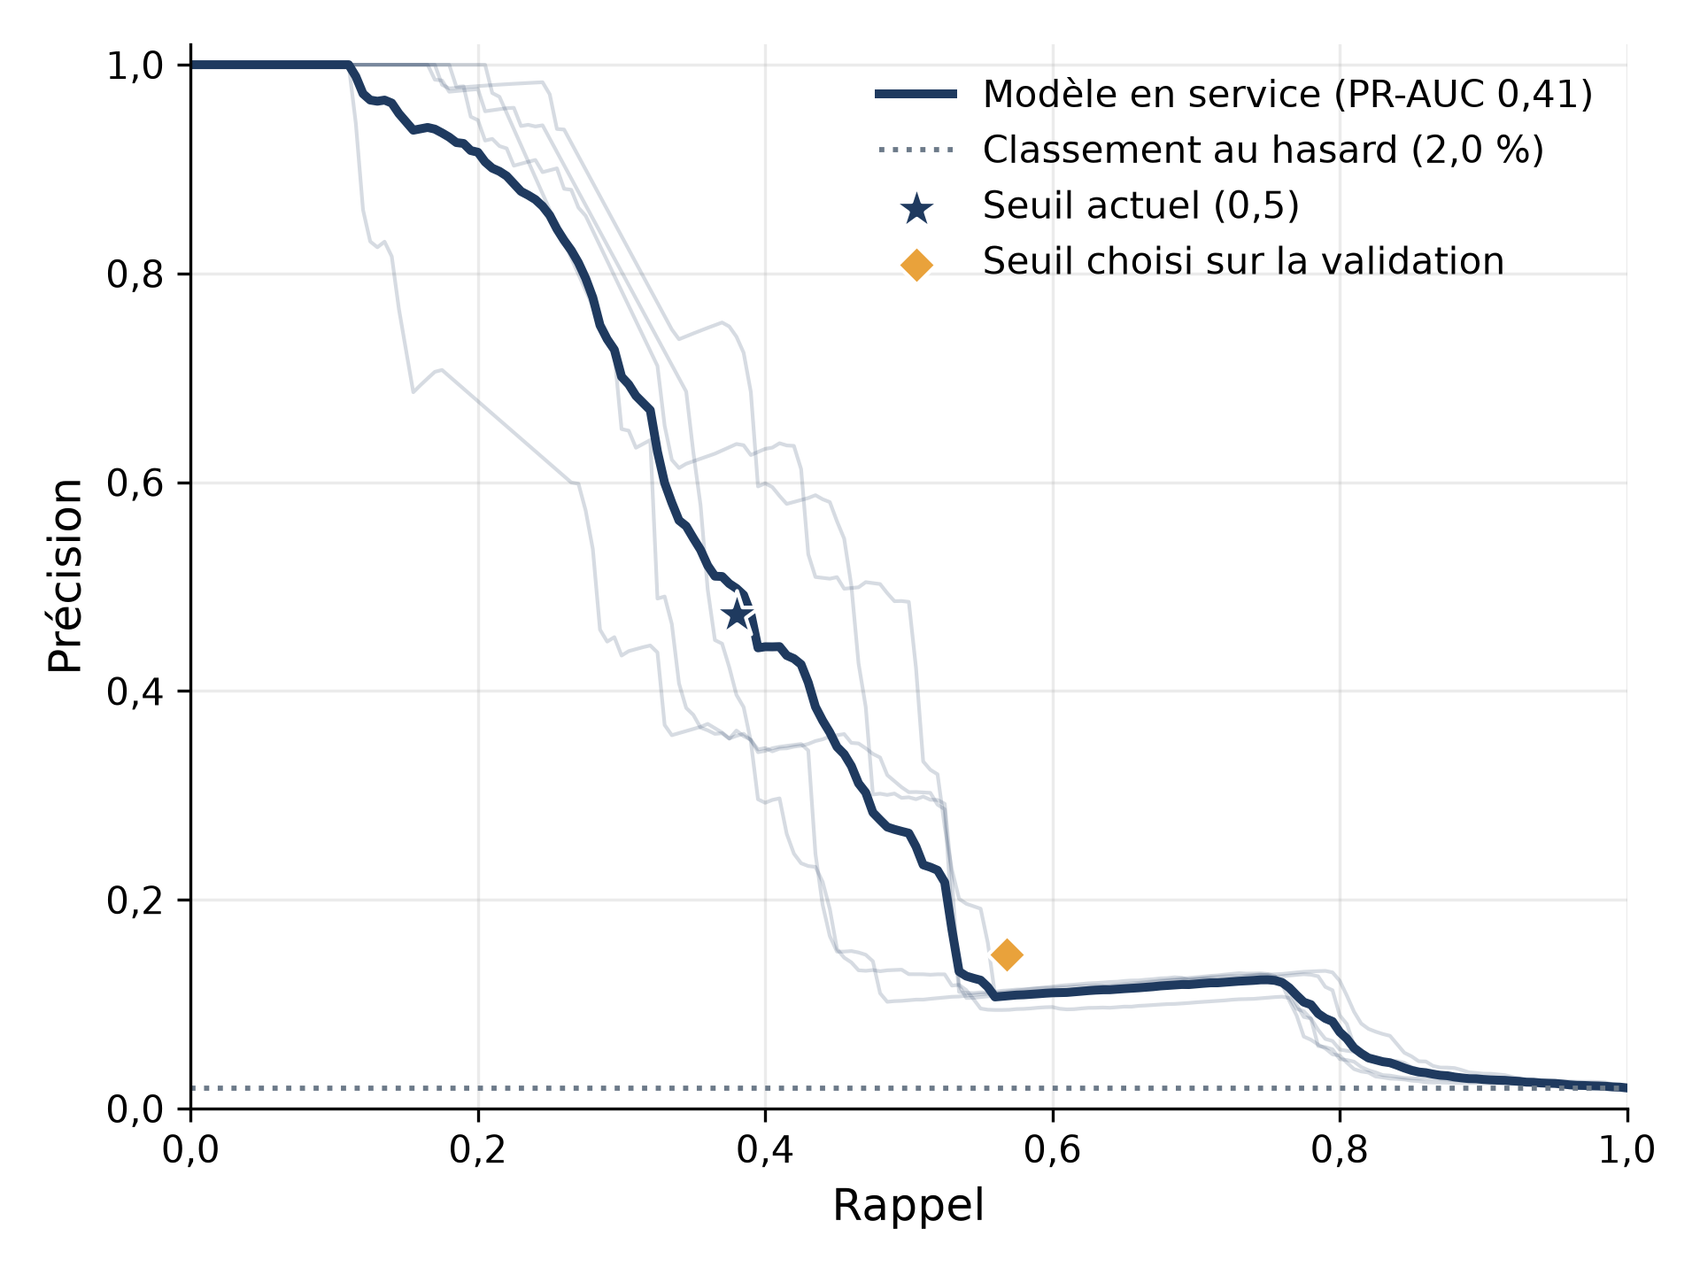
\includegraphics[width=0.75\textwidth]{fig7_pr_courbe}
\caption{Courbe précision--rappel du modèle en service sur le jeu de test}
\label{fig:pr-courbe}
\end{figure}

Recalibrer le seuil sur la validation ne constitue pas une amélioration : il donne un rappel plus élevé (0,57) mais une précision de 0,15 et 71 faux positifs pour 1\,000 fiches. La raison est instructive : la validation (juillet à septembre) ne contient pas de 13\textsuperscript{e} mois, alors que le test s'achève en décembre. Un seuil appris sur peu de mois n'est donc pas robuste, et il vaut mieux corriger la cause que recalibrer en permanence. Par ailleurs, l'ajout de la règle sur l'IBAN abaisse la PR-AUC (0,33 contre 0,41) car elle signale tous les changements d'IBAN légitimes. Un constat technique mérite d'être consigné : le seuil de 0,6 configuré dans l'application n'a en pratique aucun effet, puisque la prédiction native du modèle signale déjà tout score supérieur à 0,5. Cette décision a été mesurée telle quelle et n'a pas été modifiée.

\subsection{Détection par type d'anomalie}

La détection est très inégale selon le type (colonne \og IF en service\fg{} du tableau~\ref{tab:rappel-types}, présenté plus loin). Les anomalies qui déforment fortement le montant ou touchent l'IBAN sont presque toutes retrouvées. À l'inverse, la hausse subtile, le doublon, le salarié fantôme et le salarié sorti encore payé passent presque toujours inaperçus : la hausse de 25 à 60~\% recouvre celle des primes et promotions normales, et l'information décisive pour les deux types de salariés (absence d'historique, absence de paiement le mois précédent) ne figure pas dans les variables. Le doublon appelle une règle explicite plutôt qu'un isolement statistique.

\subsection{Sensibilité à la saisonnalité et faux positifs}

Les résultats se dégradent nettement en décembre. Avec la décision actuelle, la précision passe de 0,65 (octobre et novembre) à 0,34 en décembre, et les faux positifs pour 1\,000 fiches de 3,8 à 19,1 ; avec le seuil recalibré sur la validation, la précision tombe à 0,07 et les faux positifs montent à 193 pour 1\,000 fiches. Le 13\textsuperscript{e} mois double le montant de la fiche de trois sociétés : pour un modèle qui ne connaît pas le calendrier, c'est un montant deux fois supérieur à l'historique. Ces 13\textsuperscript{e} mois représentent 61~\% des faux positifs de la décision actuelle (66 fiches sur 108), contre 87~\% pour le seuil recalibré. Les primes ponctuelles, pourtant conçues comme des cas difficiles, génèrent très peu de fausses alertes. Presque toutes les fausses alertes proviennent donc de situations légitimes et prévisibles que le modèle ignore, ce qui oriente les améliorations.

\subsection{Comparaison des approches}

Le tableau~\ref{tab:comparaison} compare le modèle en service à d'autres approches avec le même protocole : règles métier seules, \textit{Local Outlier Factor}~\cite{breunig2000lof} et \textit{One-Class SVM}~\cite{scholkopf2001ocsvm} (deux autres algorithmes de détection d'anomalies), une combinaison de règles et du modèle, et trois variantes de l'Isolation Forest.

\begin{table}[H]
\centering
\footnotesize
\renewcommand{\arraystretch}{1.1}
\tablestyle
\begin{tabularx}{\textwidth}{|>{\raggedright\arraybackslash}p{5.6cm}|Y|Y|Y|Y|Y|}
\hline
\rowcolor{appMarine}\entete{Approche} & \entete{Précision} & \entete{Rappel} & \entete{F1} & \entete{PR-AUC} & \entete{FP / 1\,000} \\
\hline
Règles métier seules & 0,20 & 0,48 & 0,29 & 0,11 & 37,6 \\
\hline
Isolation Forest, décision en service & 0,47 & 0,38 & 0,42 & 0,41 & 8,9 \\
\hline
Isolation Forest, seuil validé & 0,15 & 0,57 & 0,23 & 0,41 & 70,8 \\
\hline
Local Outlier Factor & 0,07 & 0,17 & 0,10 & 0,06 & 49,4 \\
\hline
One-Class SVM & 0,57 & 0,47 & 0,51 & 0,45 & 7,5 \\
\hline
Règles et Isolation Forest & 0,21 & 0,56 & 0,31 & 0,15 & 41,3 \\
\hline
IF et indicateur de décembre & 0,10 & 0,58 & 0,16 & 0,33 & 129,0 \\
\hline
IF et écart relatif à la société & 0,40 & 0,54 & 0,44 & 0,51 & 19,5 \\
\hline
IF à variables retenues & 0,68 & 0,61 & 0,58 & 0,62 & 20,5 \\
\hline
\textbf{Hybride optimisé (règles et IF à variables retenues)} & \textbf{0,88} & \textbf{0,66} & \textbf{0,75} & \textbf{0,71} & \textbf{2,0} \\
\hline
\end{tabularx}
\caption{Comparaison des approches sur le jeu de test (moyenne sur cinq graines ; seuils choisis sur la validation)}
\label{tab:comparaison}
\end{table}

Quatre enseignements se dégagent de cette comparaison et de la figure~\ref{fig:comparaison}.

\begin{figure}[H]
\centering
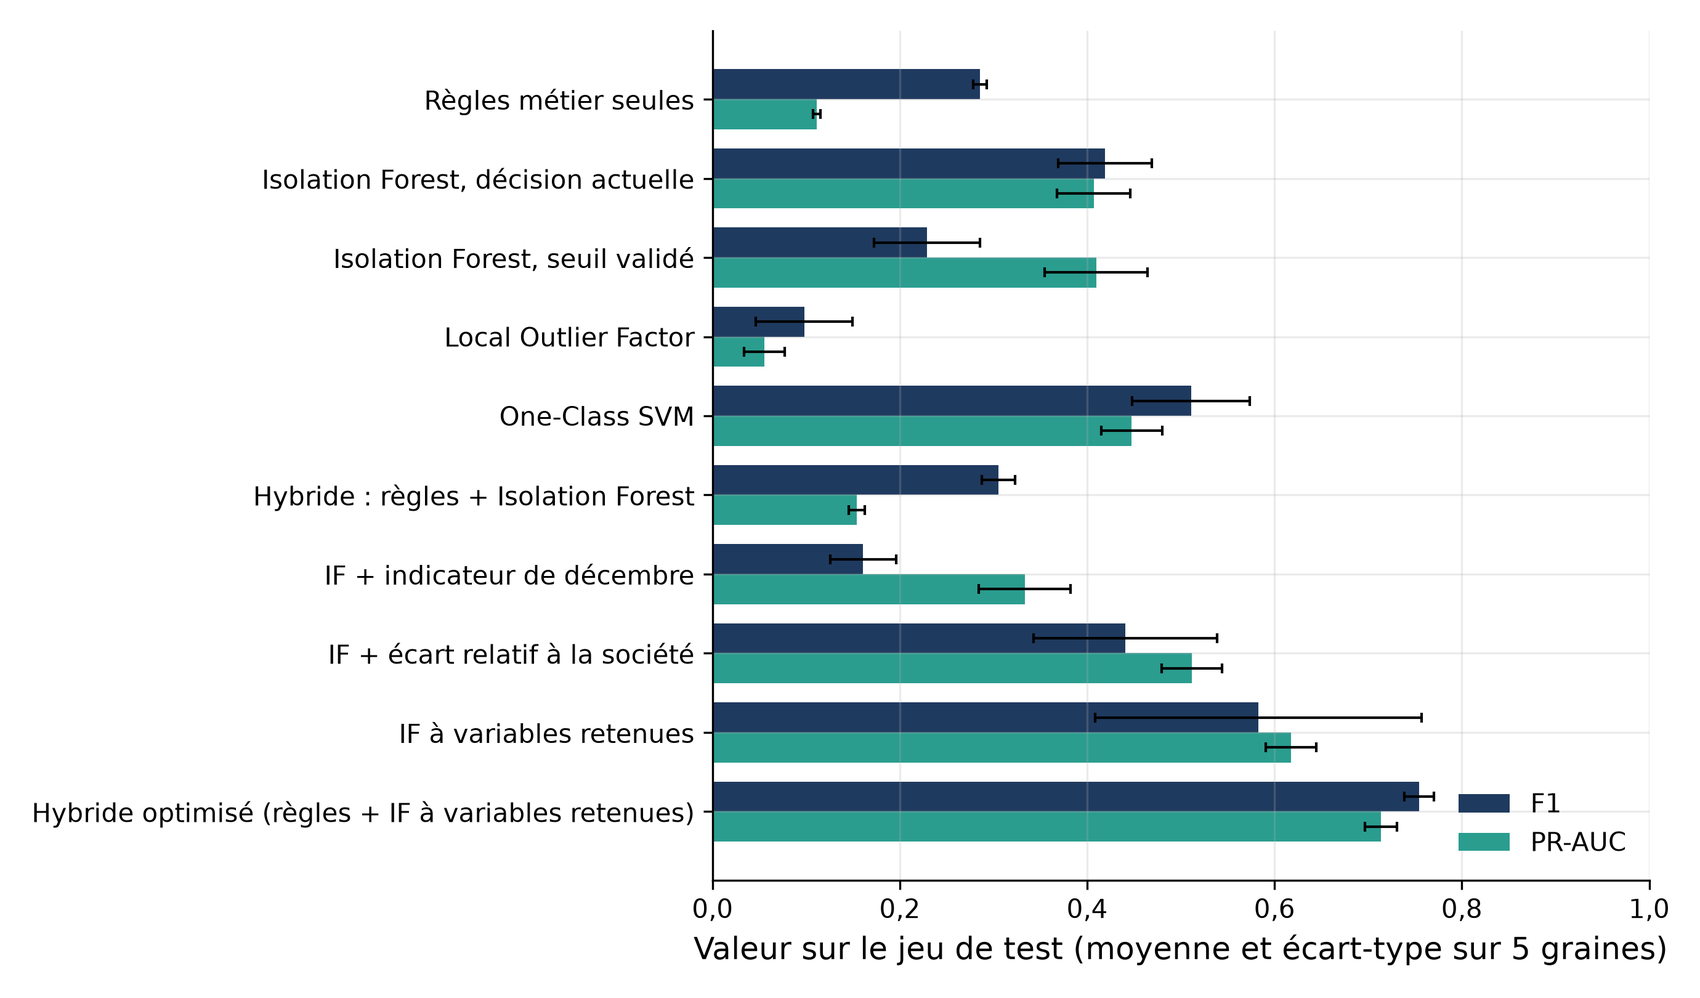
\includegraphics[width=0.9\textwidth]{fig7_comparaison}
\caption{F1 et PR-AUC de chaque approche sur le jeu de test (barres : écart-type sur cinq graines)}
\label{fig:comparaison}
\end{figure}

\begin{itemize}
    \item \textbf{L'algorithme n'est pas le facteur déterminant.} Le One-Class SVM, entraîné en une fraction de seconde, fait aussi bien que l'Isolation Forest (F1 de 0,51), tandis que le \textit{Local Outlier Factor} est presque au niveau du hasard et peut être écarté. Les temps de calcul sont négligeables pour toutes les approches.
    \item \textbf{Un indicateur de décembre dégrade le résultat} (F1 de 0,16 contre 0,23). Avec un seul mois de décembre à l'entraînement, il isole ce mois entier au lieu de décrire le comportement des sociétés concernées.
    \item \textbf{Une variable qui exprime la cause vaut mieux qu'une variable qui désigne la période.} Rapporter l'écart de chaque salarié à celui de sa société pour le mois traite l'effet collectif d'un 13\textsuperscript{e} mois sans connaître le calendrier : le F1 passe à 0,44 et la PR-AUC à 0,51.
    \item \textbf{La combinaison de règles et d'un modèle à variables sélectionnées est la plus performante.} Elle atteint un F1 de 0,75, une PR-AUC de 0,71 et deux faux positifs pour 1\,000 fiches, avec une grande stabilité entre graines (écart-type de 0,02), car les règles détectent avec certitude une partie des anomalies.
\end{itemize}

\subsection{Ablation des variables}

Pour comprendre quelles variables servent le modèle, on a retiré chacune d'elles successivement et mesuré la variation de la PR-AUC (tableau~\ref{tab:ablation}). Retirer une variable utile dégrade la performance ; retirer une variable nuisible l'améliore.

\begin{table}[H]
\centering
\small
\renewcommand{\arraystretch}{1.15}
\tablestyle
\begin{tabularx}{\textwidth}{|>{\raggedright\arraybackslash}p{5.6cm}|Y|Y|Y|Y|}
\hline
\rowcolor{appMarine}\entete{Variable retirée} & \entete{PR-AUC (test)} & \entete{Variation (test)} & \entete{PR-AUC (validation)} & \entete{Variation (validation)} \\
\hline
Aucune (modèle complet) & 0,41 & -- & 0,59 & -- \\
\hline
Montant & 0,51 & +0,10 & 0,69 & +0,10 \\
\hline
Écart à la moyenne du salarié & 0,38 & $-$0,03 & 0,49 & $-$0,10 \\
\hline
Écart dans le lot (\textit{z-score}) & 0,46 & +0,05 & 0,69 & +0,11 \\
\hline
Variation sur le mois précédent & 0,36 & $-$0,05 & 0,48 & $-$0,10 \\
\hline
IBAN modifié & 0,35 & $-$0,06 & 0,54 & $-$0,05 \\
\hline
Paiements sur le même IBAN & 0,38 & $-$0,03 & 0,49 & $-$0,09 \\
\hline
\end{tabularx}
\caption{Ablation des variables de l'Isolation Forest (moyenne sur cinq graines)}
\label{tab:ablation}
\end{table}

Le montant brut et l'écart dans le lot sont nuisibles : leur retrait améliore la PR-AUC, car le montant seul est peu informatif lorsque les salaires vont de 1\,500 à plus de 10\,000~\texteuro{}. L'indicateur d'IBAN modifié, la variation sur le mois précédent, l'écart à la moyenne du salarié et le nombre de paiements sur le même IBAN sont utiles. Les mêmes variables ressortent sur la validation et sur le test : la sélection a été faite sur la validation seule, sans observer le test.

\subsection{Valeur ajoutée de l'IA face aux règles}

La question centrale est celle de la complémentarité. Sur environ 241 anomalies par jeu de test, la figure~\ref{fig:valeur-ajoutee} répartit chaque type selon le détecteur qui le retrouve.

\begin{figure}[H]
\centering
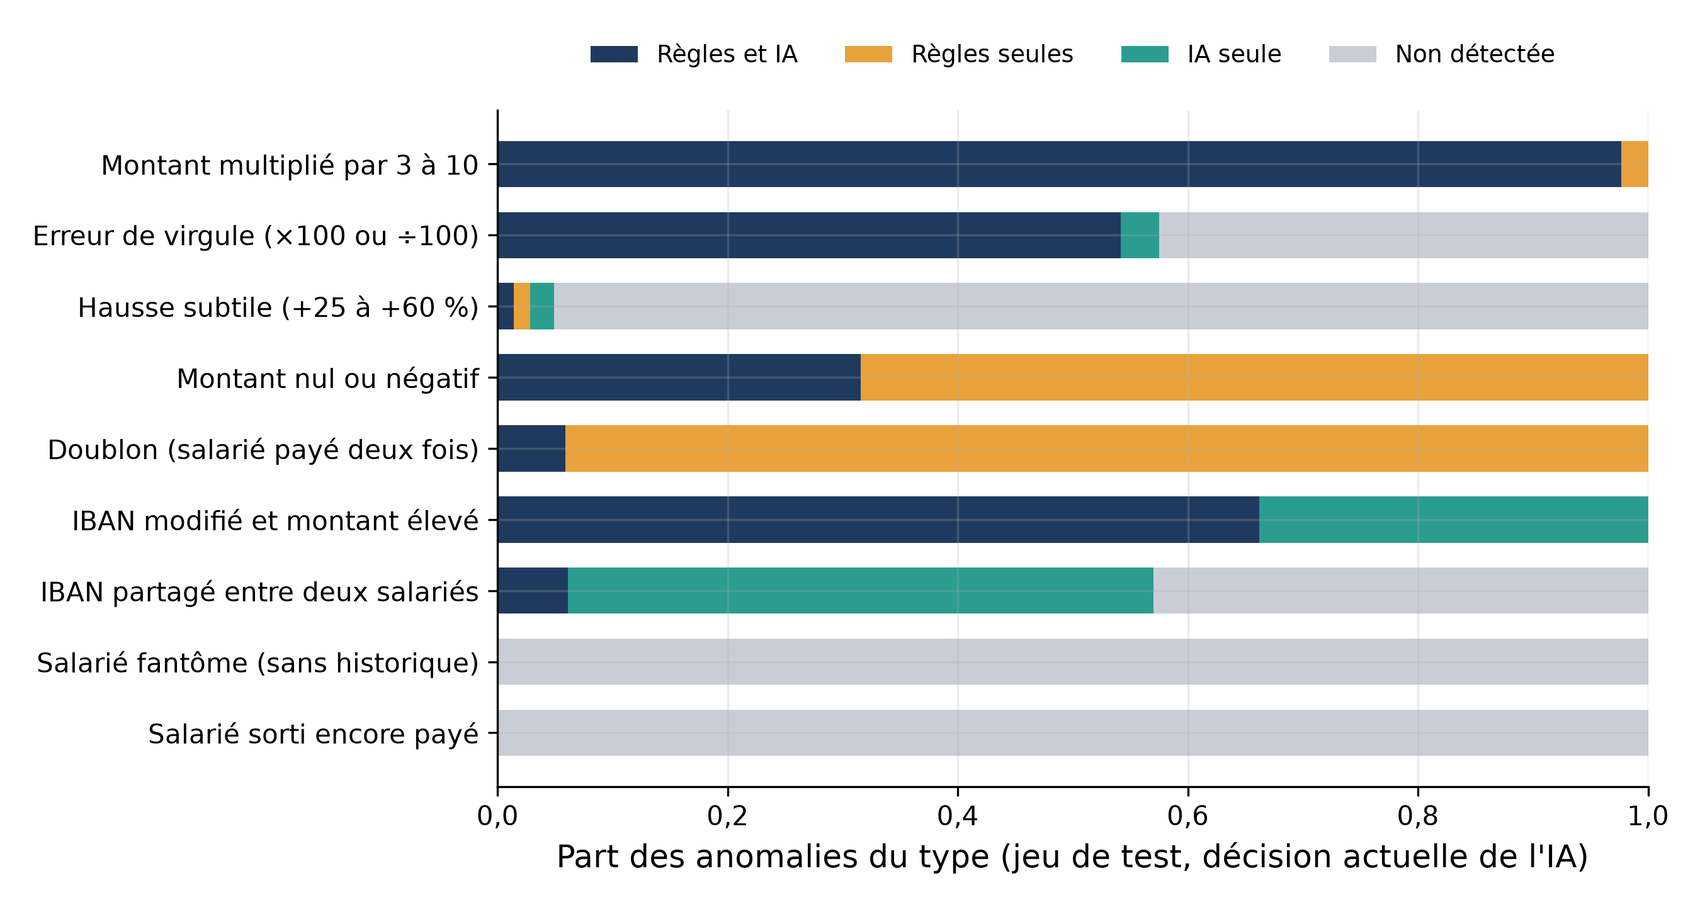
\includegraphics[width=0.92\textwidth]{fig7_valeur_ajoutee}
\caption{Répartition des anomalies de chaque type selon le détecteur (règles, IA, les deux, aucun)}
\label{fig:valeur-ajoutee}
\end{figure}

En moyenne par graine, 22 anomalies sont vues par l'IA seule, soit 16~\% des anomalies détectées, contre 47 vues par les règles seules et 69 par les deux ; 102 échappent aux deux. L'IA apporte surtout sur les IBAN partagés, les IBAN modifiés avec montant élevé et les erreurs de virgule. Les règles sont irremplaçables pour les doublons et les montants nuls ou négatifs, qu'un modèle statistique distingue mal. En contrepartie, les règles produisent 423 fausses alertes que l'IA ne partage pas (les 13\textsuperscript{e} mois), contre 72 pour l'IA seule. Aucun des deux détecteurs ne suffit seul : ce résultat justifie une approche hybride.

Le tableau~\ref{tab:rappel-types} détaille le rappel par type pour les principales approches, et conclut ces comparaisons. Les règles atteignent un rappel complet sur les doublons et les montants nuls ; l'Isolation Forest et le One-Class SVM sont meilleurs sur les IBAN modifiés et partagés. La suppression du montant brut rend la hausse subtile détectable (63 à 75~\% contre 3~\%), et l'hybride optimisé atteint 100~\% sur quatre autres types. Deux types restent à 0~\% quelle que soit l'approche : le salarié fantôme et le salarié sorti encore payé. Ils appellent des informations nouvelles (historique de présence, registre du personnel) plutôt qu'un algorithme différent.

\begin{table}[H]
\centering
\footnotesize
\renewcommand{\arraystretch}{1.15}
\tablestyle
\begin{tabularx}{\textwidth}{|>{\raggedright\arraybackslash}p{3.9cm}|Y|Y|Y|Y|Y|Y|}
\hline
\rowcolor{appMarine}\entete{Type d'anomalie} & \entete{Règles seules} & \entete{IF en service} & \entete{One-Class SVM} & \entete{Règles et IF} & \entete{IF retenues} & \entete{Hybride optimisé} \\
\hline
Montant multiplié par 3 à 10 & 100 & 98 & 88 & 100 & 100 & 100 \\
\hline
Erreur de virgule & 54 & 57 & 67 & 70 & 100 & 100 \\
\hline
Hausse subtile & 3 & 3 & 1 & 6 & 75 & 63 \\
\hline
Montant nul ou négatif & 100 & 28 & 66 & 100 & 100 & 100 \\
\hline
Doublon & 100 & 6 & 79 & 100 & 26 & 100 \\
\hline
IBAN modifié et montant élevé & 66 & 100 & 43 & 88 & 100 & 100 \\
\hline
IBAN partagé & 7 & 57 & 92 & 37 & 49 & 32 \\
\hline
Salarié fantôme & 0 & 0 & 0 & 0 & 0 & 0 \\
\hline
Salarié sorti encore payé & 0 & 0 & 0 & 0 & 0 & 0 \\
\hline
\end{tabularx}
\caption{Taux de détection (en \%) par type d'anomalie et par approche, jeu de test}
\label{tab:rappel-types}
\end{table}

\subsection{Modèle candidat et choix retenu}

Sur la base de ces résultats, l'approche recommandée est l'\textbf{hybride optimisé} : des règles métier (IBAN invalide, montant non positif, doublon, montant supérieur à deux fois l'écart relatif à la société) combinées à un Isolation Forest sur cinq variables, dont l'écart relatif à la société et sans le montant brut ni l'écart dans le lot. Sur le test, il détecte 66~\% des anomalies avec une précision de 88~\%, contre 38~\% et 47~\% pour la décision actuelle, et réduit les faux positifs de neuf à deux pour 1\,000 fiches. Son seuil et ses variables ont été choisis sur la validation seule ; il est aussi le meilleur sur la validation.

Cette version a été préparée comme \textbf{modèle candidat} avec ses métadonnées, mais elle n'a \textbf{pas été activée} : le modèle en service reste inchangé. Ce choix prudent s'explique par les limites exposées ci-dessous : une mise en service suppose de valider le gain sur des données réelles lors d'un pilote. Il illustre aussi l'intérêt d'une évaluation séparée du déploiement : l'équipe peut améliorer le modèle sans modifier le comportement de l'application.

\subsection{Scénario de démonstration}

Pour présenter le comportement de l'application sur un cas concret, un fichier de 1\,100 fiches contenant 12 anomalies connues a été constitué (annexe~\ref{ann:scenario}). Le tableau~\ref{tab:scenario} indique ce que l'application signale avec le modèle en service.

\begin{table}[H]
\centering
\footnotesize
\renewcommand{\arraystretch}{1.0}
\tablestyle
\begin{tabularx}{\textwidth}{|>{\raggedright\arraybackslash}p{4.8cm}|>{\raggedright\arraybackslash}p{3cm}|Y|}
\hline
\rowcolor{appMarine}\entete{Anomalie connue} & \entete{Contrôle IA} & \entete{Autre contrôle} \\
\hline
Montant multiplié par 3 à 10 & Oui, élevé (0,75) & -- \\
\hline
Erreur de virgule ($\times$100) & Oui, élevé (0,87) & -- \\
\hline
Erreur de virgule ($\div$100) & Non & -- \\
\hline
Hausse subtile & Oui, moyen (0,54) & -- \\
\hline
IBAN modifié et montant élevé & Oui, élevé (0,60) & -- \\
\hline
IBAN partagé (première fiche) & Oui, élevé (0,60) & -- \\
\hline
IBAN partagé (seconde fiche) & Non & -- \\
\hline
Montant nul ou négatif & Non & Contrôle métier : erreur \\
\hline
Doublon (deux fiches) & Non & Contrôle métier : avertissement \\
\hline
Salarié fantôme & Non & -- \\
\hline
Salarié sorti encore payé & Non & -- \\
\hline
\end{tabularx}
\caption{Scénario de démonstration : 12 fiches anormales connues parmi 1\,100}
\label{tab:scenario}
\end{table}

Le contrôle IA signale neuf fiches sur 1\,100 (0,8~\%), dont cinq sont de vraies anomalies parmi les 12 connues. Les contrôles métier complètent ce résultat en signalant le montant nul et le doublon, que l'IA seule ne voit pas. Quatre signalements sont de fausses alertes : trois changements d'IBAN légitimes, que la règle sur l'IBAN signale systématiquement pour vérification, et une fiche au profil inhabituel. Quatre anomalies restent non détectées, conformément aux limites mesurées. Ce scénario illustre l'apport de l'IA sans en cacher les limites.

\subsection{Limites et validité des résultats}

Les résultats doivent être interprétés avec prudence :
\begin{itemize}
    \item les données sont \textbf{synthétiques} et les anomalies sont injectées selon des règles connues, ce qui peut favoriser les approches qui exploitent les mêmes signaux ; les résultats mesurent la capacité à retrouver des anomalies plausibles, non la performance sur de vraies paies ;
    \item l'historique est supposé correct, et les salaires suivent des lois simples ;
    \item le jeu de test compte de 22 à 35 fiches par type : c'est pourquoi les mesures sont répétées sur cinq graines, et les écarts entre variantes proches ne doivent pas être sur-interprétés ;
    \item l'entraînement ne contient qu'un seul mois de décembre, ce qui limite l'apprentissage du 13\textsuperscript{e} mois ;
    \item le modèle candidat n'a pas été éprouvé en conditions réelles et n'est pas déployé.
\end{itemize}
Les performances sur des données de production devront être confirmées par un pilote, et le seuil fixé avec les utilisateurs, en arbitrant entre anomalies manquées et temps de vérification.

\section{Tests et validation}

Les tests du sprint, résumés dans le tableau~\ref{tab:tests-s4}, s'exécutent avec succès : 27 tests Python et 12 tests du backend. Les tests de l'évaluation vérifient aussi la rigueur du protocole, par exemple que le seuil est bien choisi sur la validation seule et que le découpage chronologique ne produit aucune fuite d'information.

\begin{table}[H]
\centering
\footnotesize
\renewcommand{\arraystretch}{1.1}
\tablestyle
\begin{tabularx}{\textwidth}{|>{\raggedright\arraybackslash}p{3.6cm}|Y|>{\centering\arraybackslash}p{1.3cm}|}
\hline
\rowcolor{appMarine}\entete{Domaine} & \entete{Comportements vérifiés} & \entete{Tests} \\
\hline
Variables et explications (Python) & Écart à la moyenne avec et sans historique ; IBAN partagé et \textit{z-score} ; types probables ; distinction doublon / IBAN partagé ; une recommandation par type ; contrat de l'interface & 9 \\
\hline
Service de détection (Python) & État du module ; signalement d'un montant suspect ; lot vide & 3 \\
\hline
Métriques et règle IBAN (Python) & Évaluation complète ; règle \og IBAN modifié\fg{} ; compatibilité du générateur ; rapport de métriques & 4 \\
\hline
Évaluation reproductible (Python) & Jeu de données : volumétrie, IBAN valides, découpage sans fuite, déterminisme, scénario ; protocole : seuil choisi sur la validation, décision en service ; règles de comparaison ; candidat non activé & 11 \\
\hline
Intégration non bloquante (backend) & IA désactivée sans appel ; marquage d'une fiche suspecte ; erreur du module sans exception ; niveaux de risque & 4 \\
\hline
Supervision et indicateurs (backend) & Précision observée ; réentraînement réel excluant les anomalies confirmées et refusé si trop peu de paiements ; source inconnue ; indicateurs de l'apport de l'IA & 8 \\
\hline
\end{tabularx}
\caption{Tests automatisés du sprint 4}
\label{tab:tests-s4}
\end{table}

\section{Conclusion}

Le sprint 4 a livré une détection par intelligence artificielle intégrée à l'application sans la fragiliser : un module indépendant, non bloquant, dont chaque signalement est expliqué et assorti d'une recommandation. Son évaluation, menée avec un protocole rigoureux, montre ce que le modèle en service apporte et ce qu'il ne fait pas : il retrouve environ 38~\% des anomalies avec une précision de 47~\%, excelle sur les erreurs qui déforment le montant ou l'IBAN, et reste aveugle à plusieurs types. Elle montre surtout que le gain vient moins de l'algorithme que des variables et de la combinaison avec les règles : un hybride optimisé atteint un F1 de 0,75. Ces résultats, obtenus sur des données synthétiques, devront être confirmés sur des données réelles avant toute mise en service du modèle candidat. Le chapitre suivant présente le dernier sprint, consacré au pilotage, au déploiement et à la recette.
